\chapter{CONTROL REGION PLOTS}
\label{appendixB}

The control regions defined by the \VHbb\ analysis are used to validate the agreement between data and Monte-Carlo (MC) simulation.

\begin{figure}[htbp]
  \centering
  \mbox{
    \subfigure [] {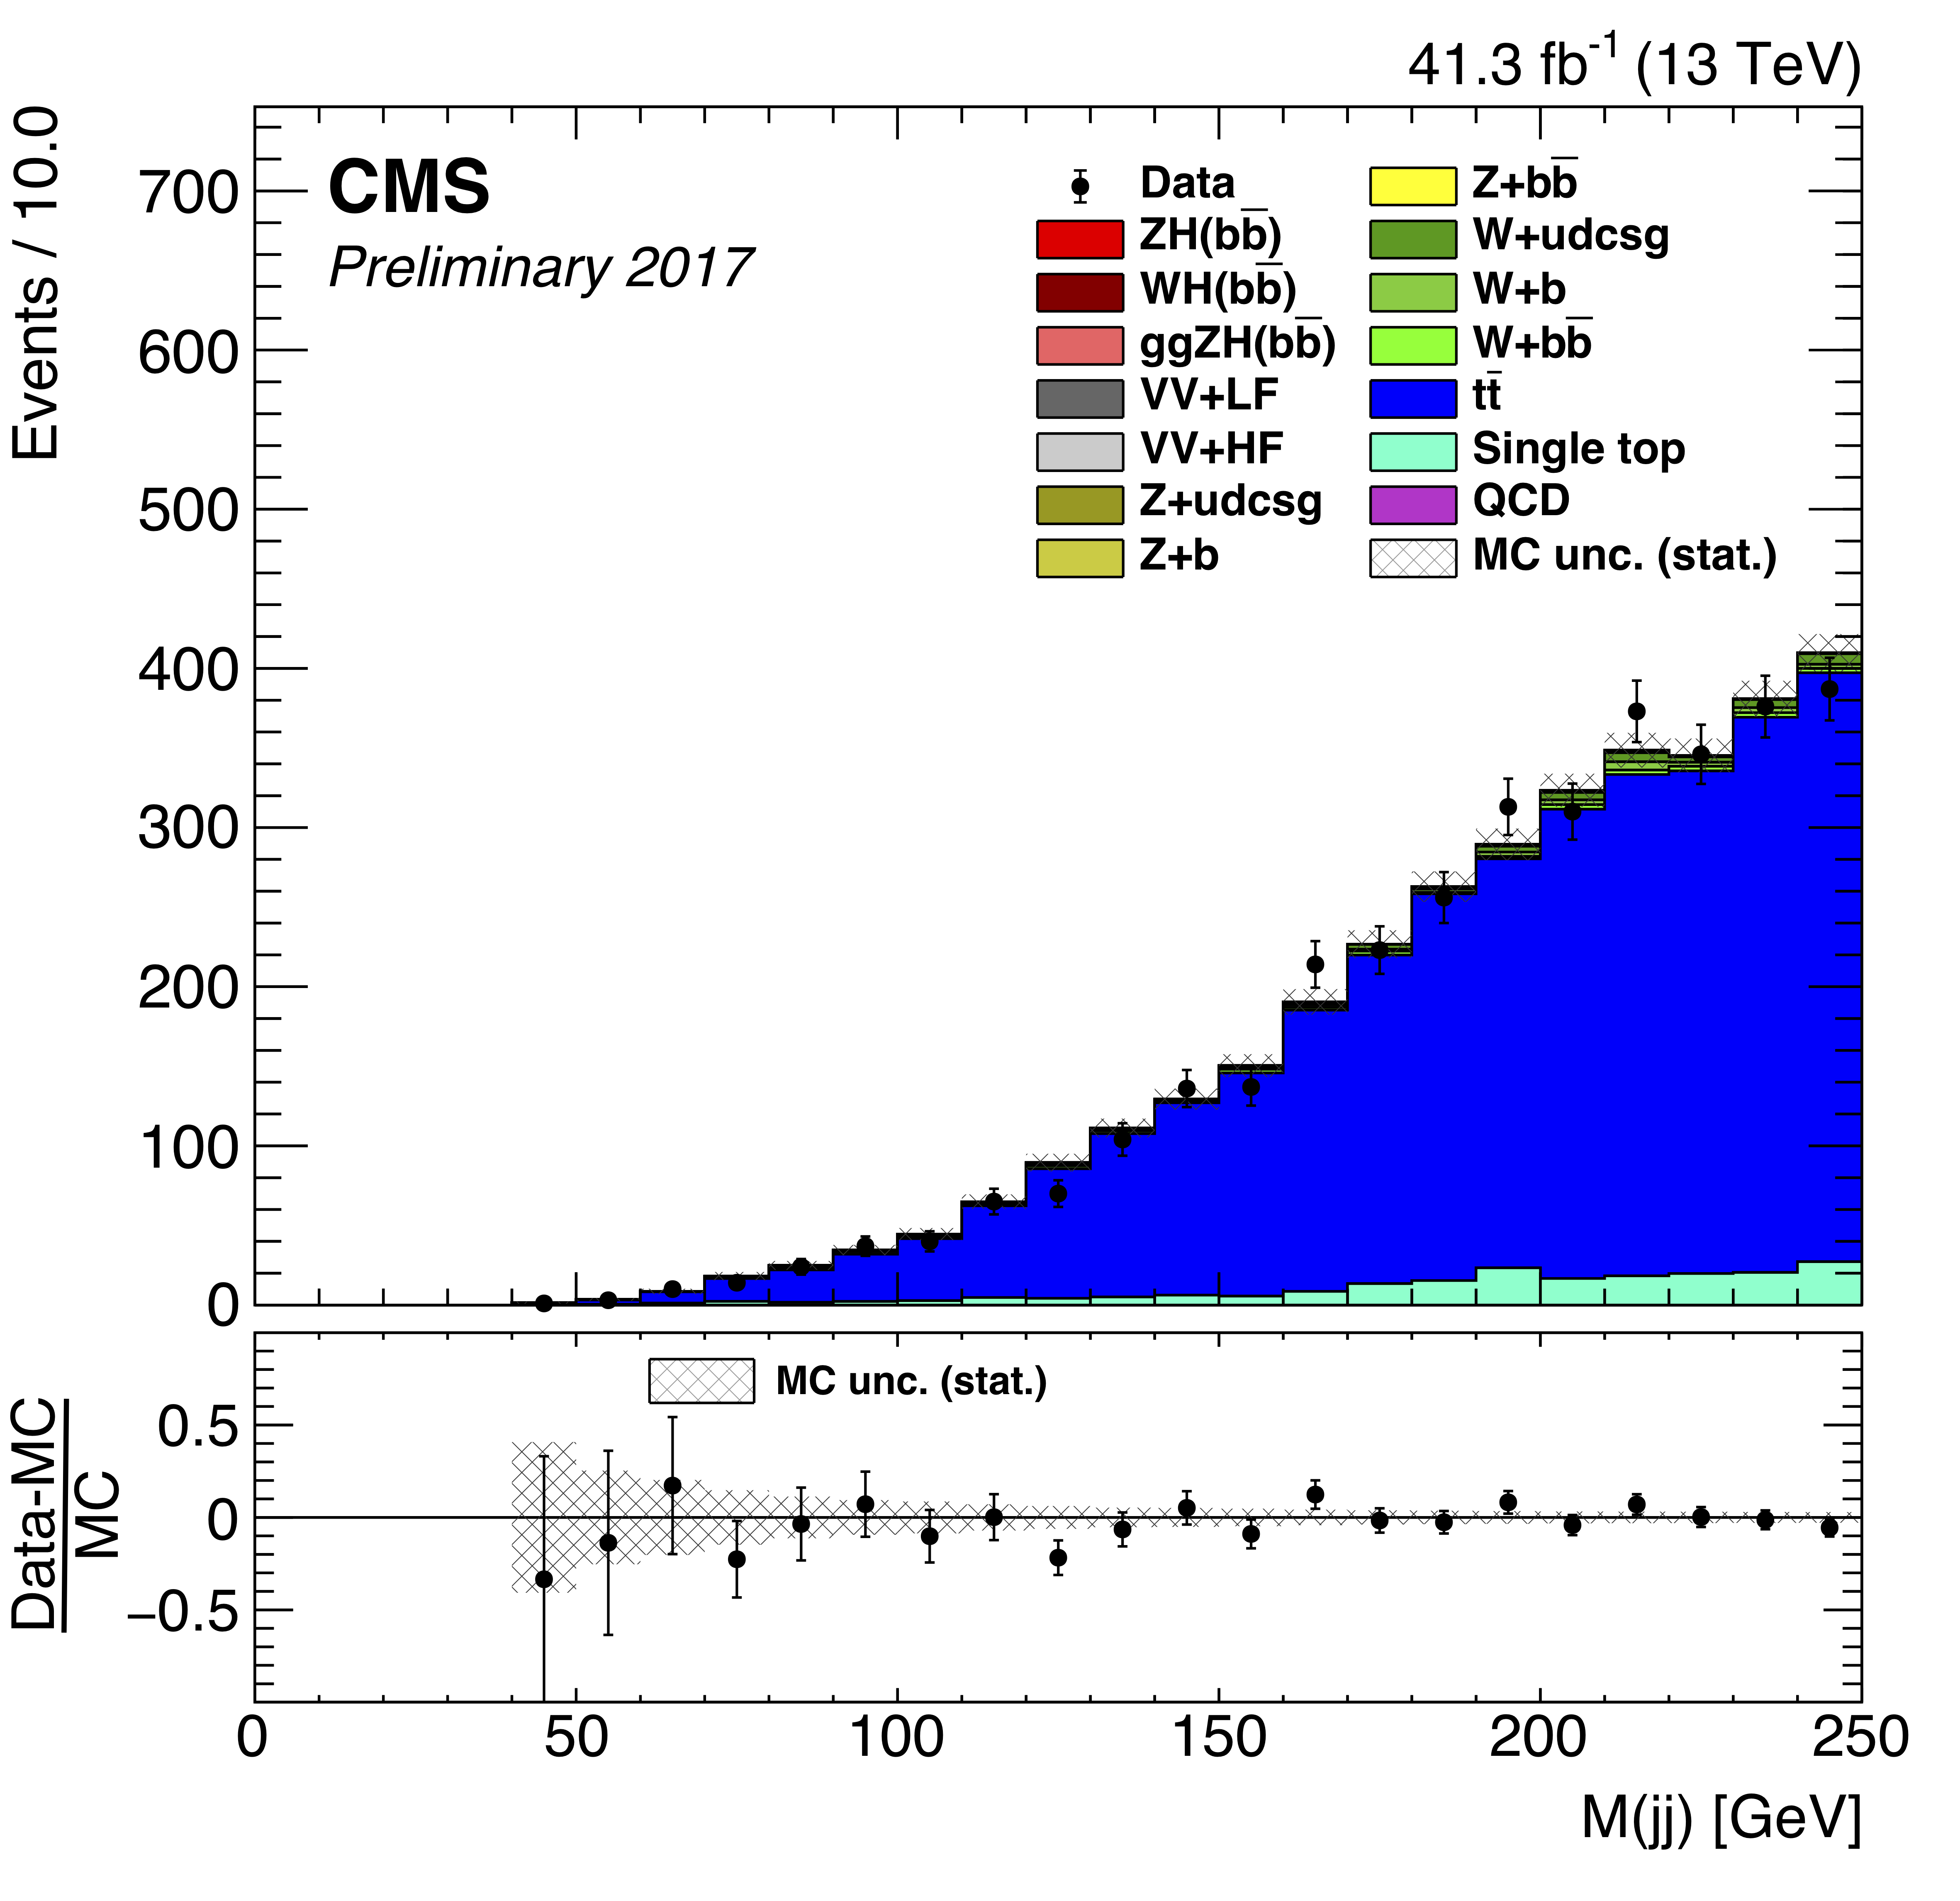
\includegraphics[width=0.4\linewidth]{images/CR_Znn_TT/H_mass}}
    \subfigure [] {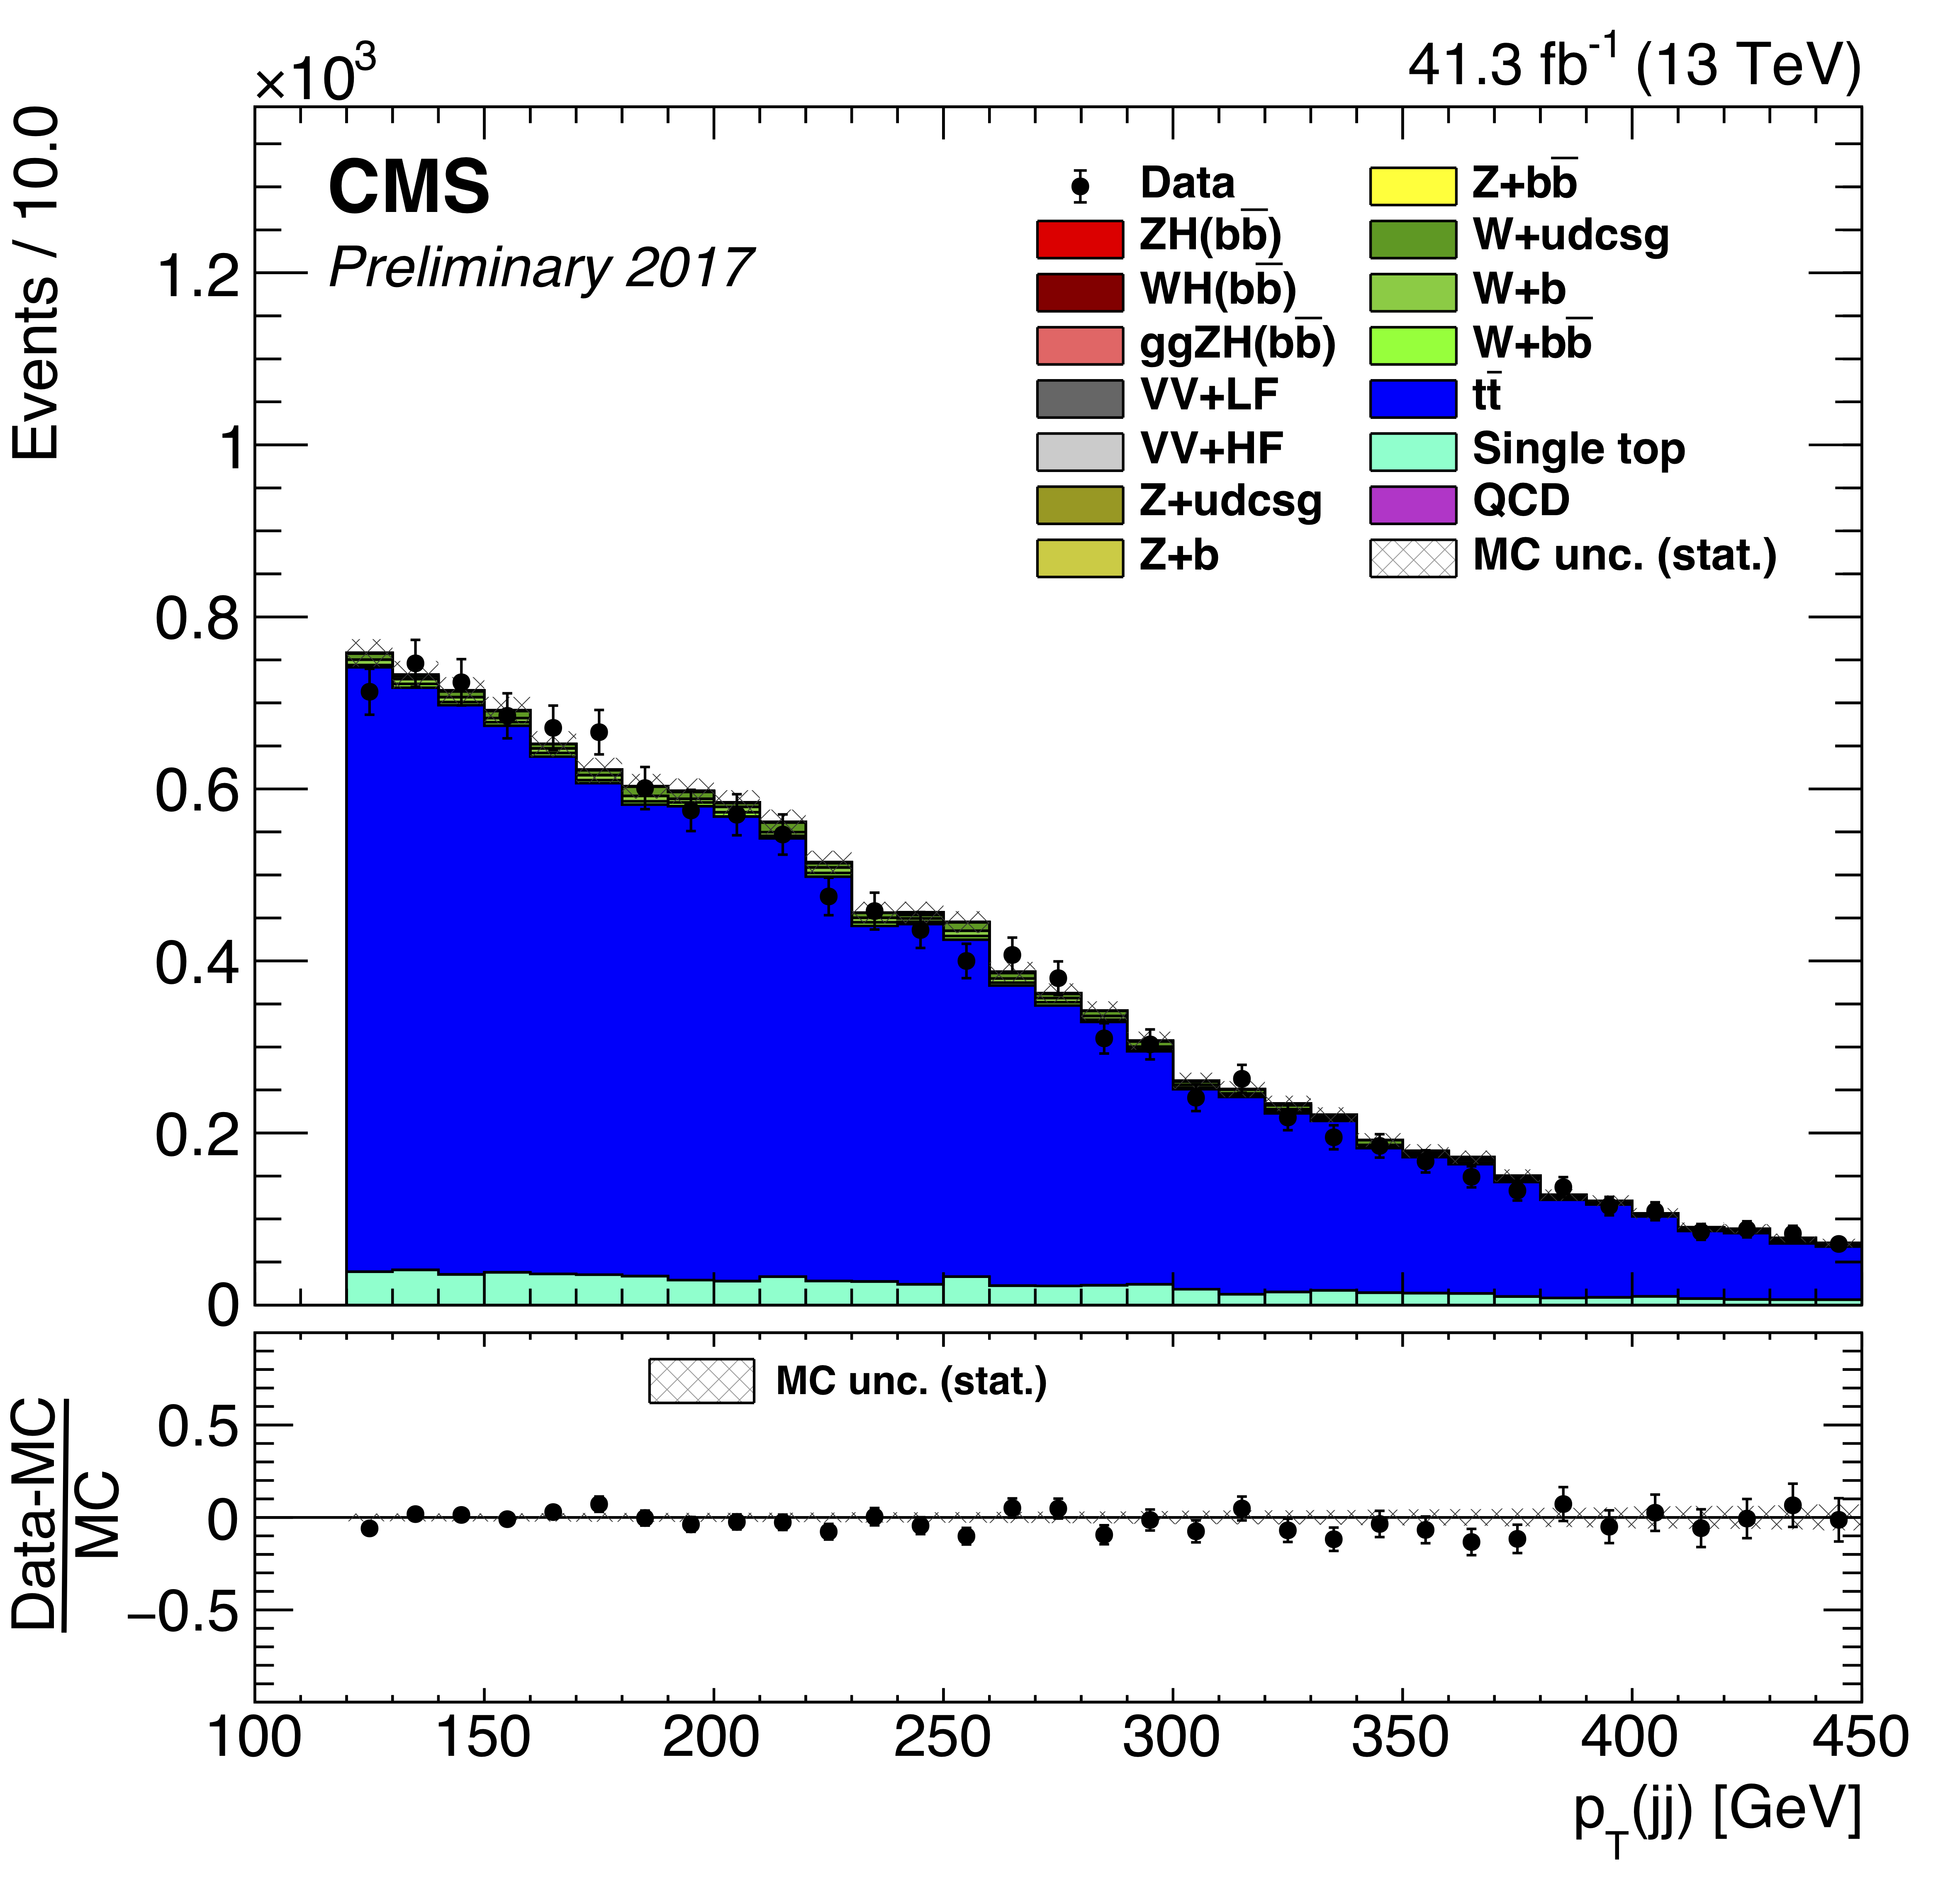
\includegraphics[width=0.4\linewidth]{images/CR_Znn_TT/H_pt}}
  }
  \mbox{
    \subfigure [] {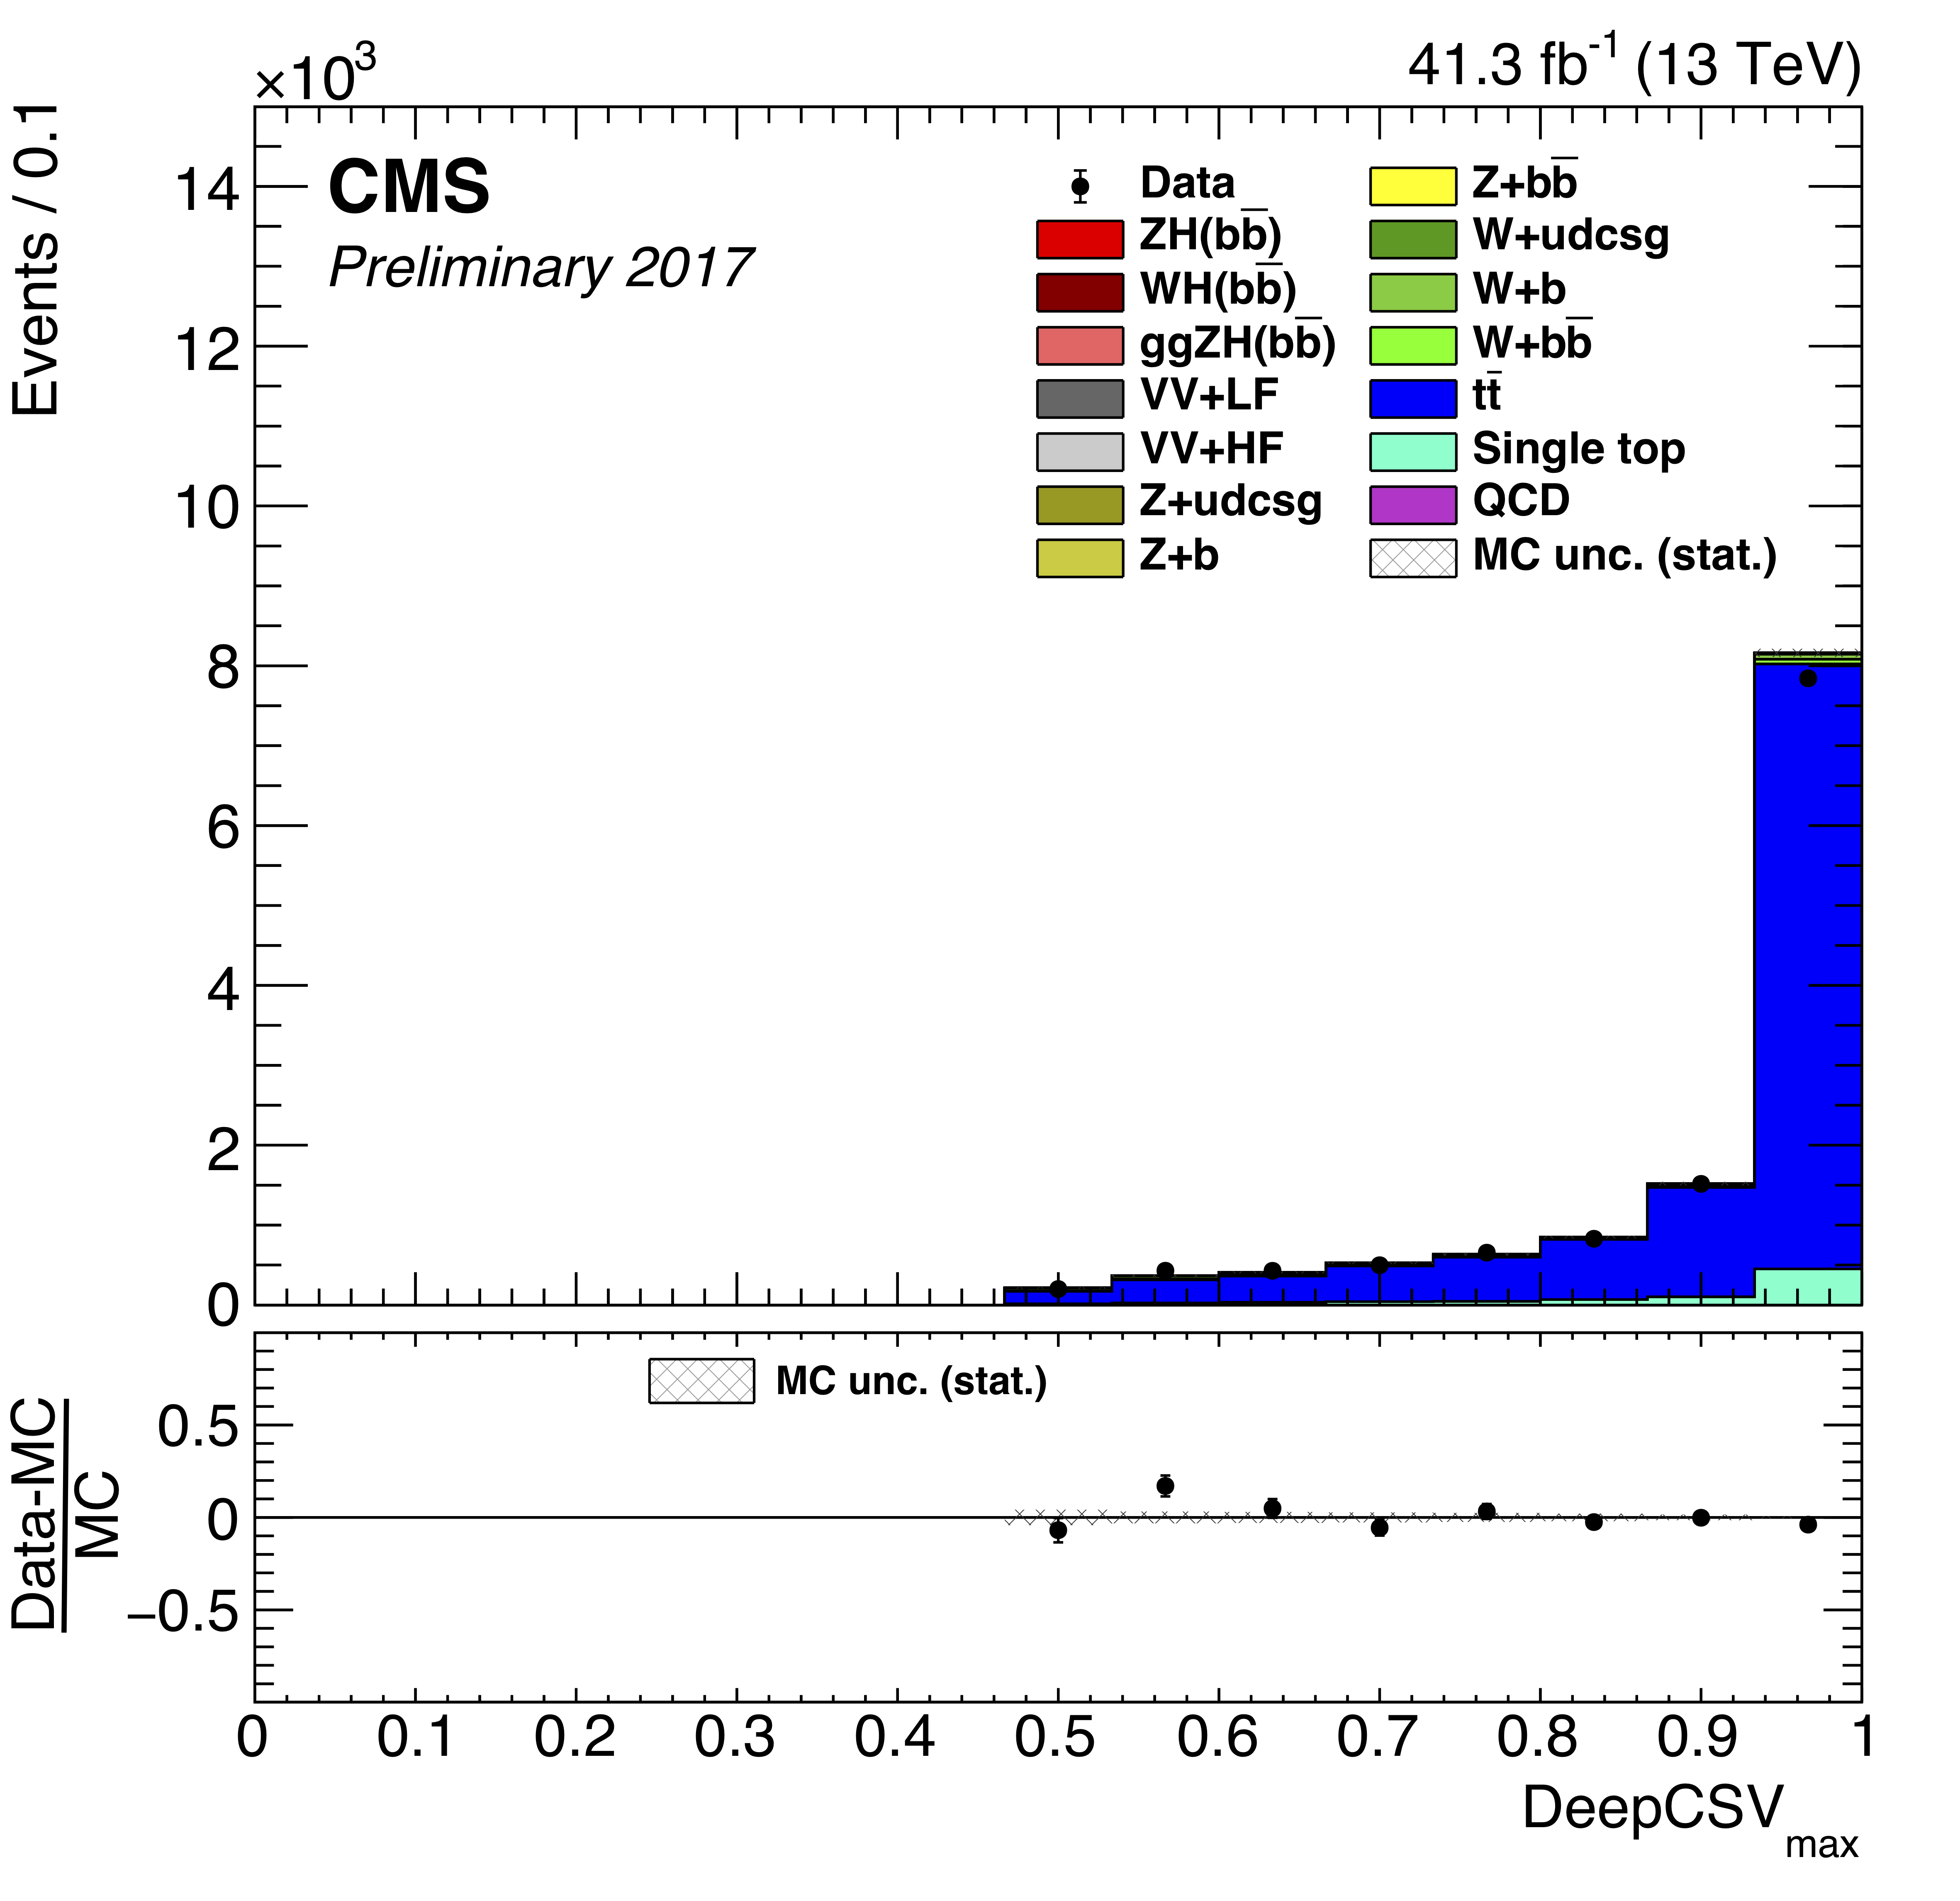
\includegraphics[width=0.4\linewidth]{images/CR_Znn_TT/hJets_DeepCSV_0}}
    \subfigure [] {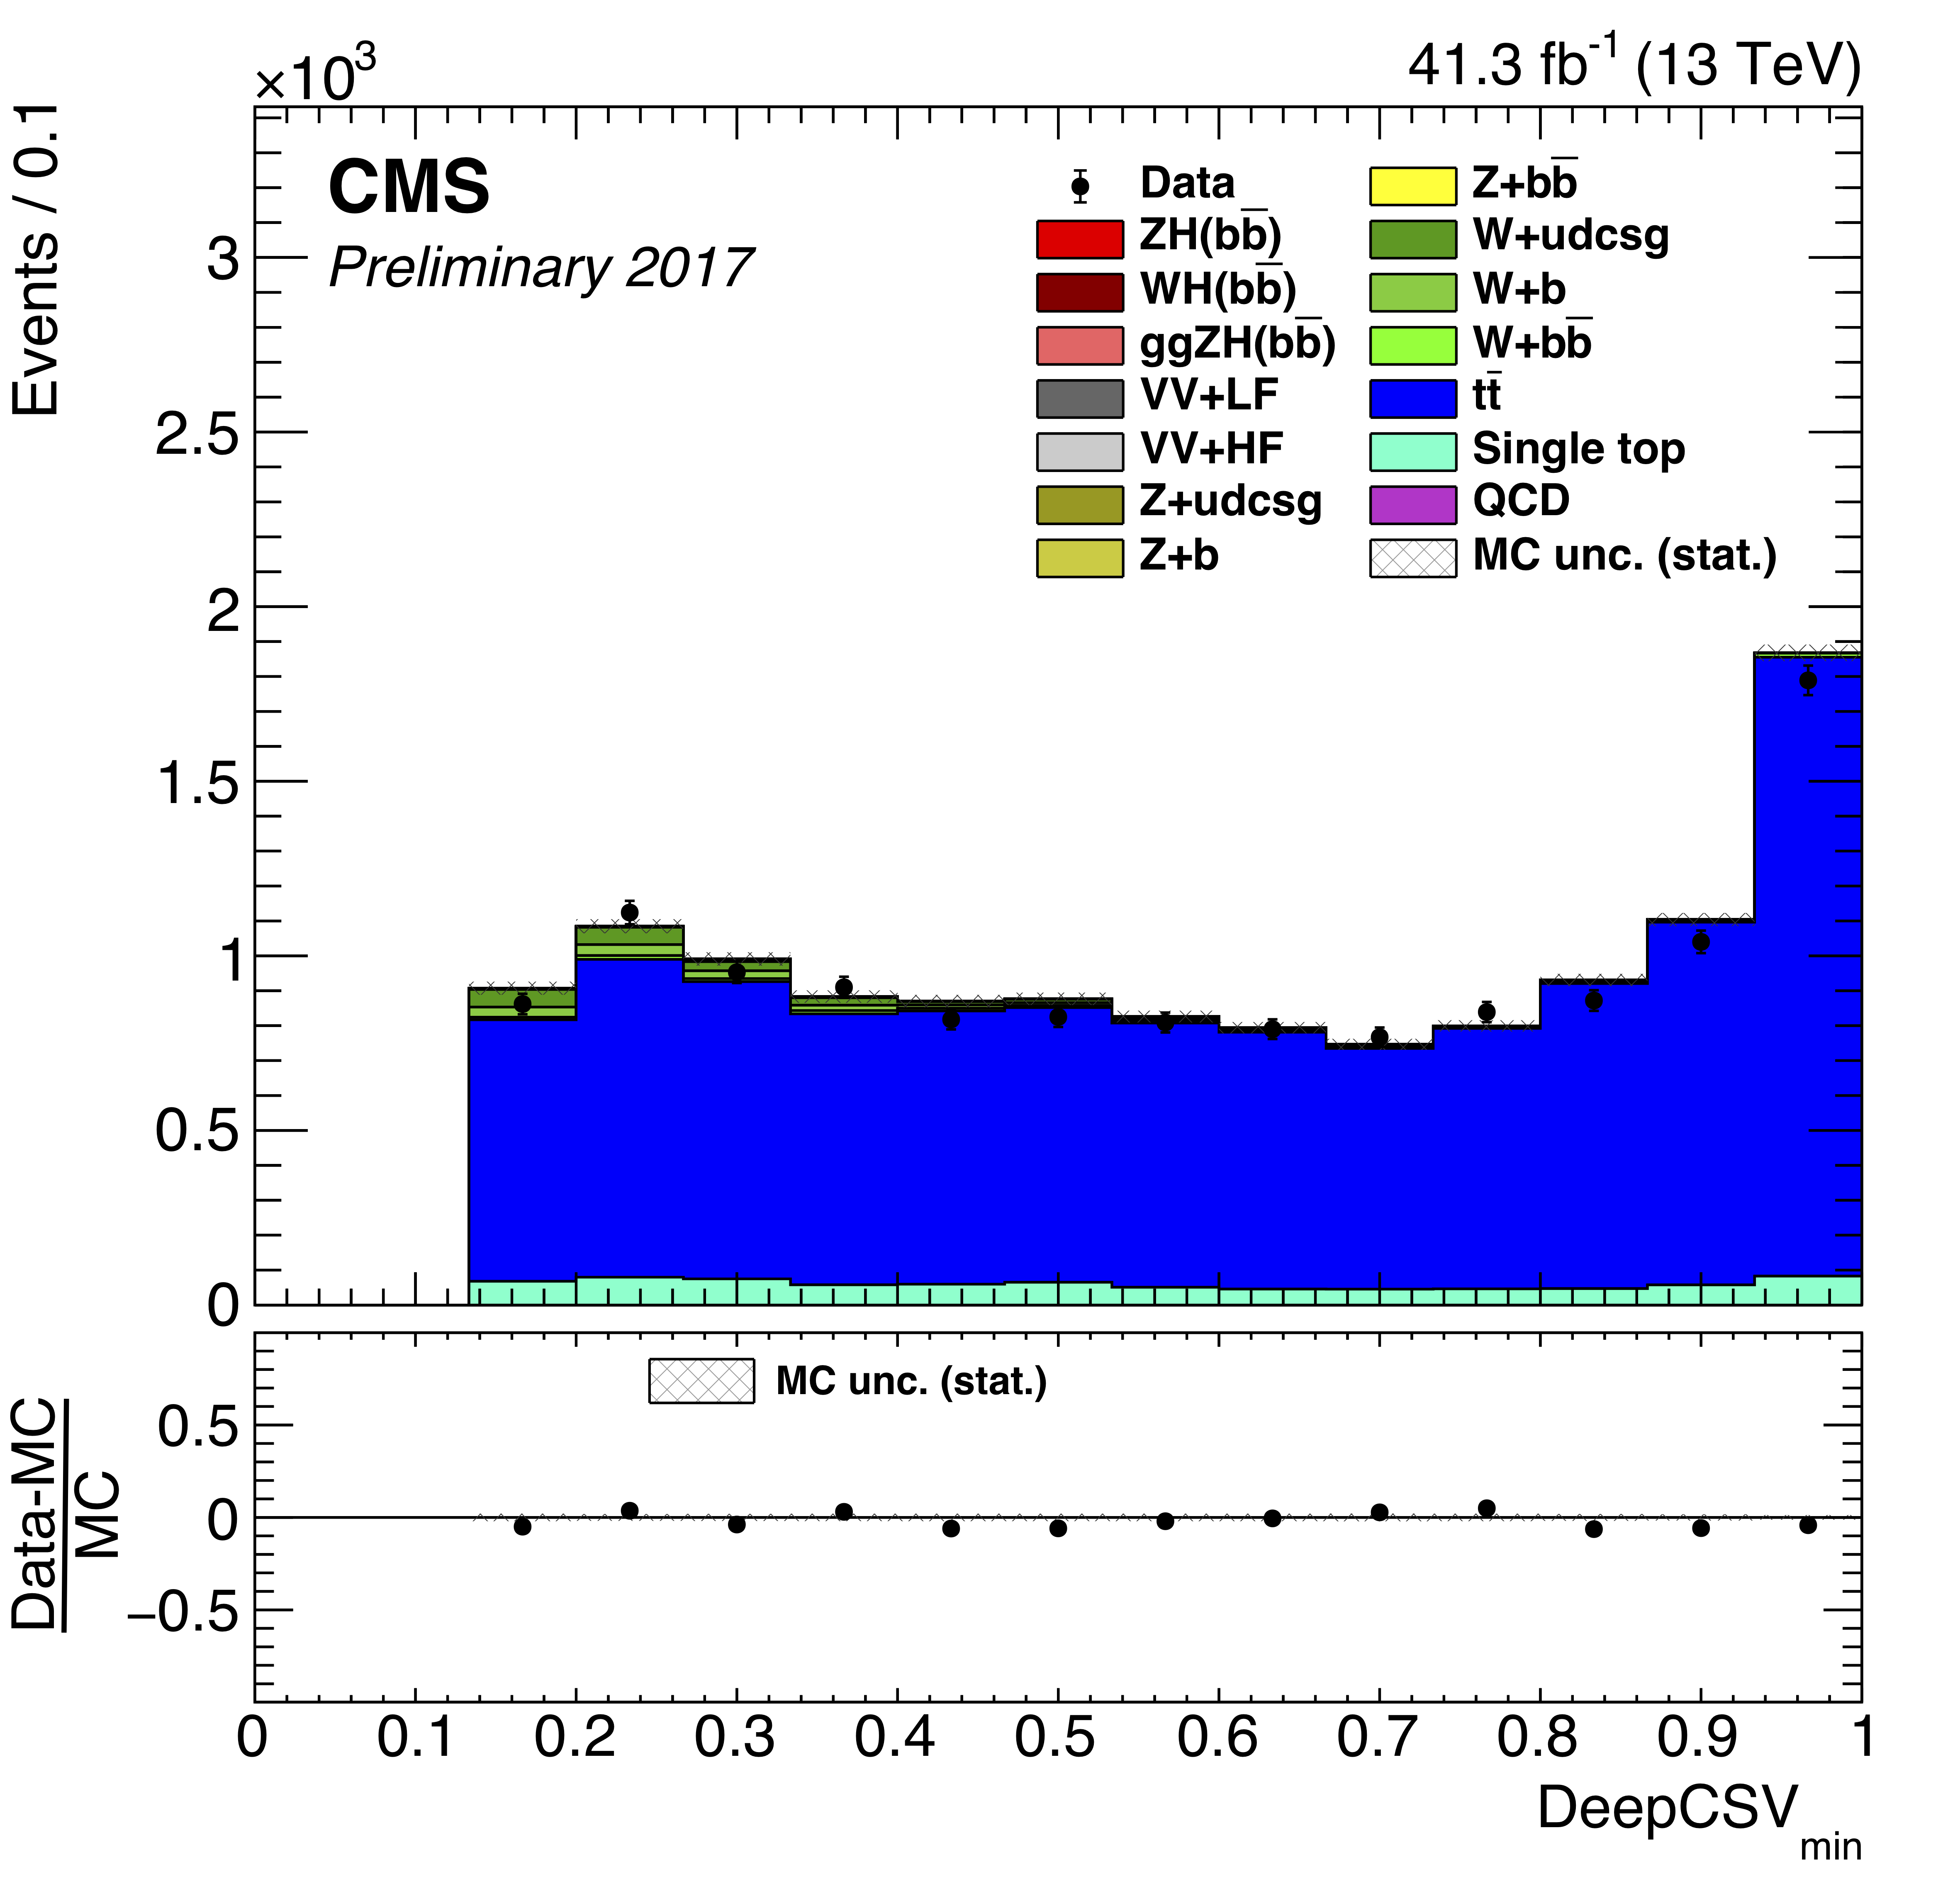
\includegraphics[width=0.4\linewidth]{images/CR_Znn_TT/hJets_DeepCSV_1}}
  }
  \mbox{
    \subfigure [] {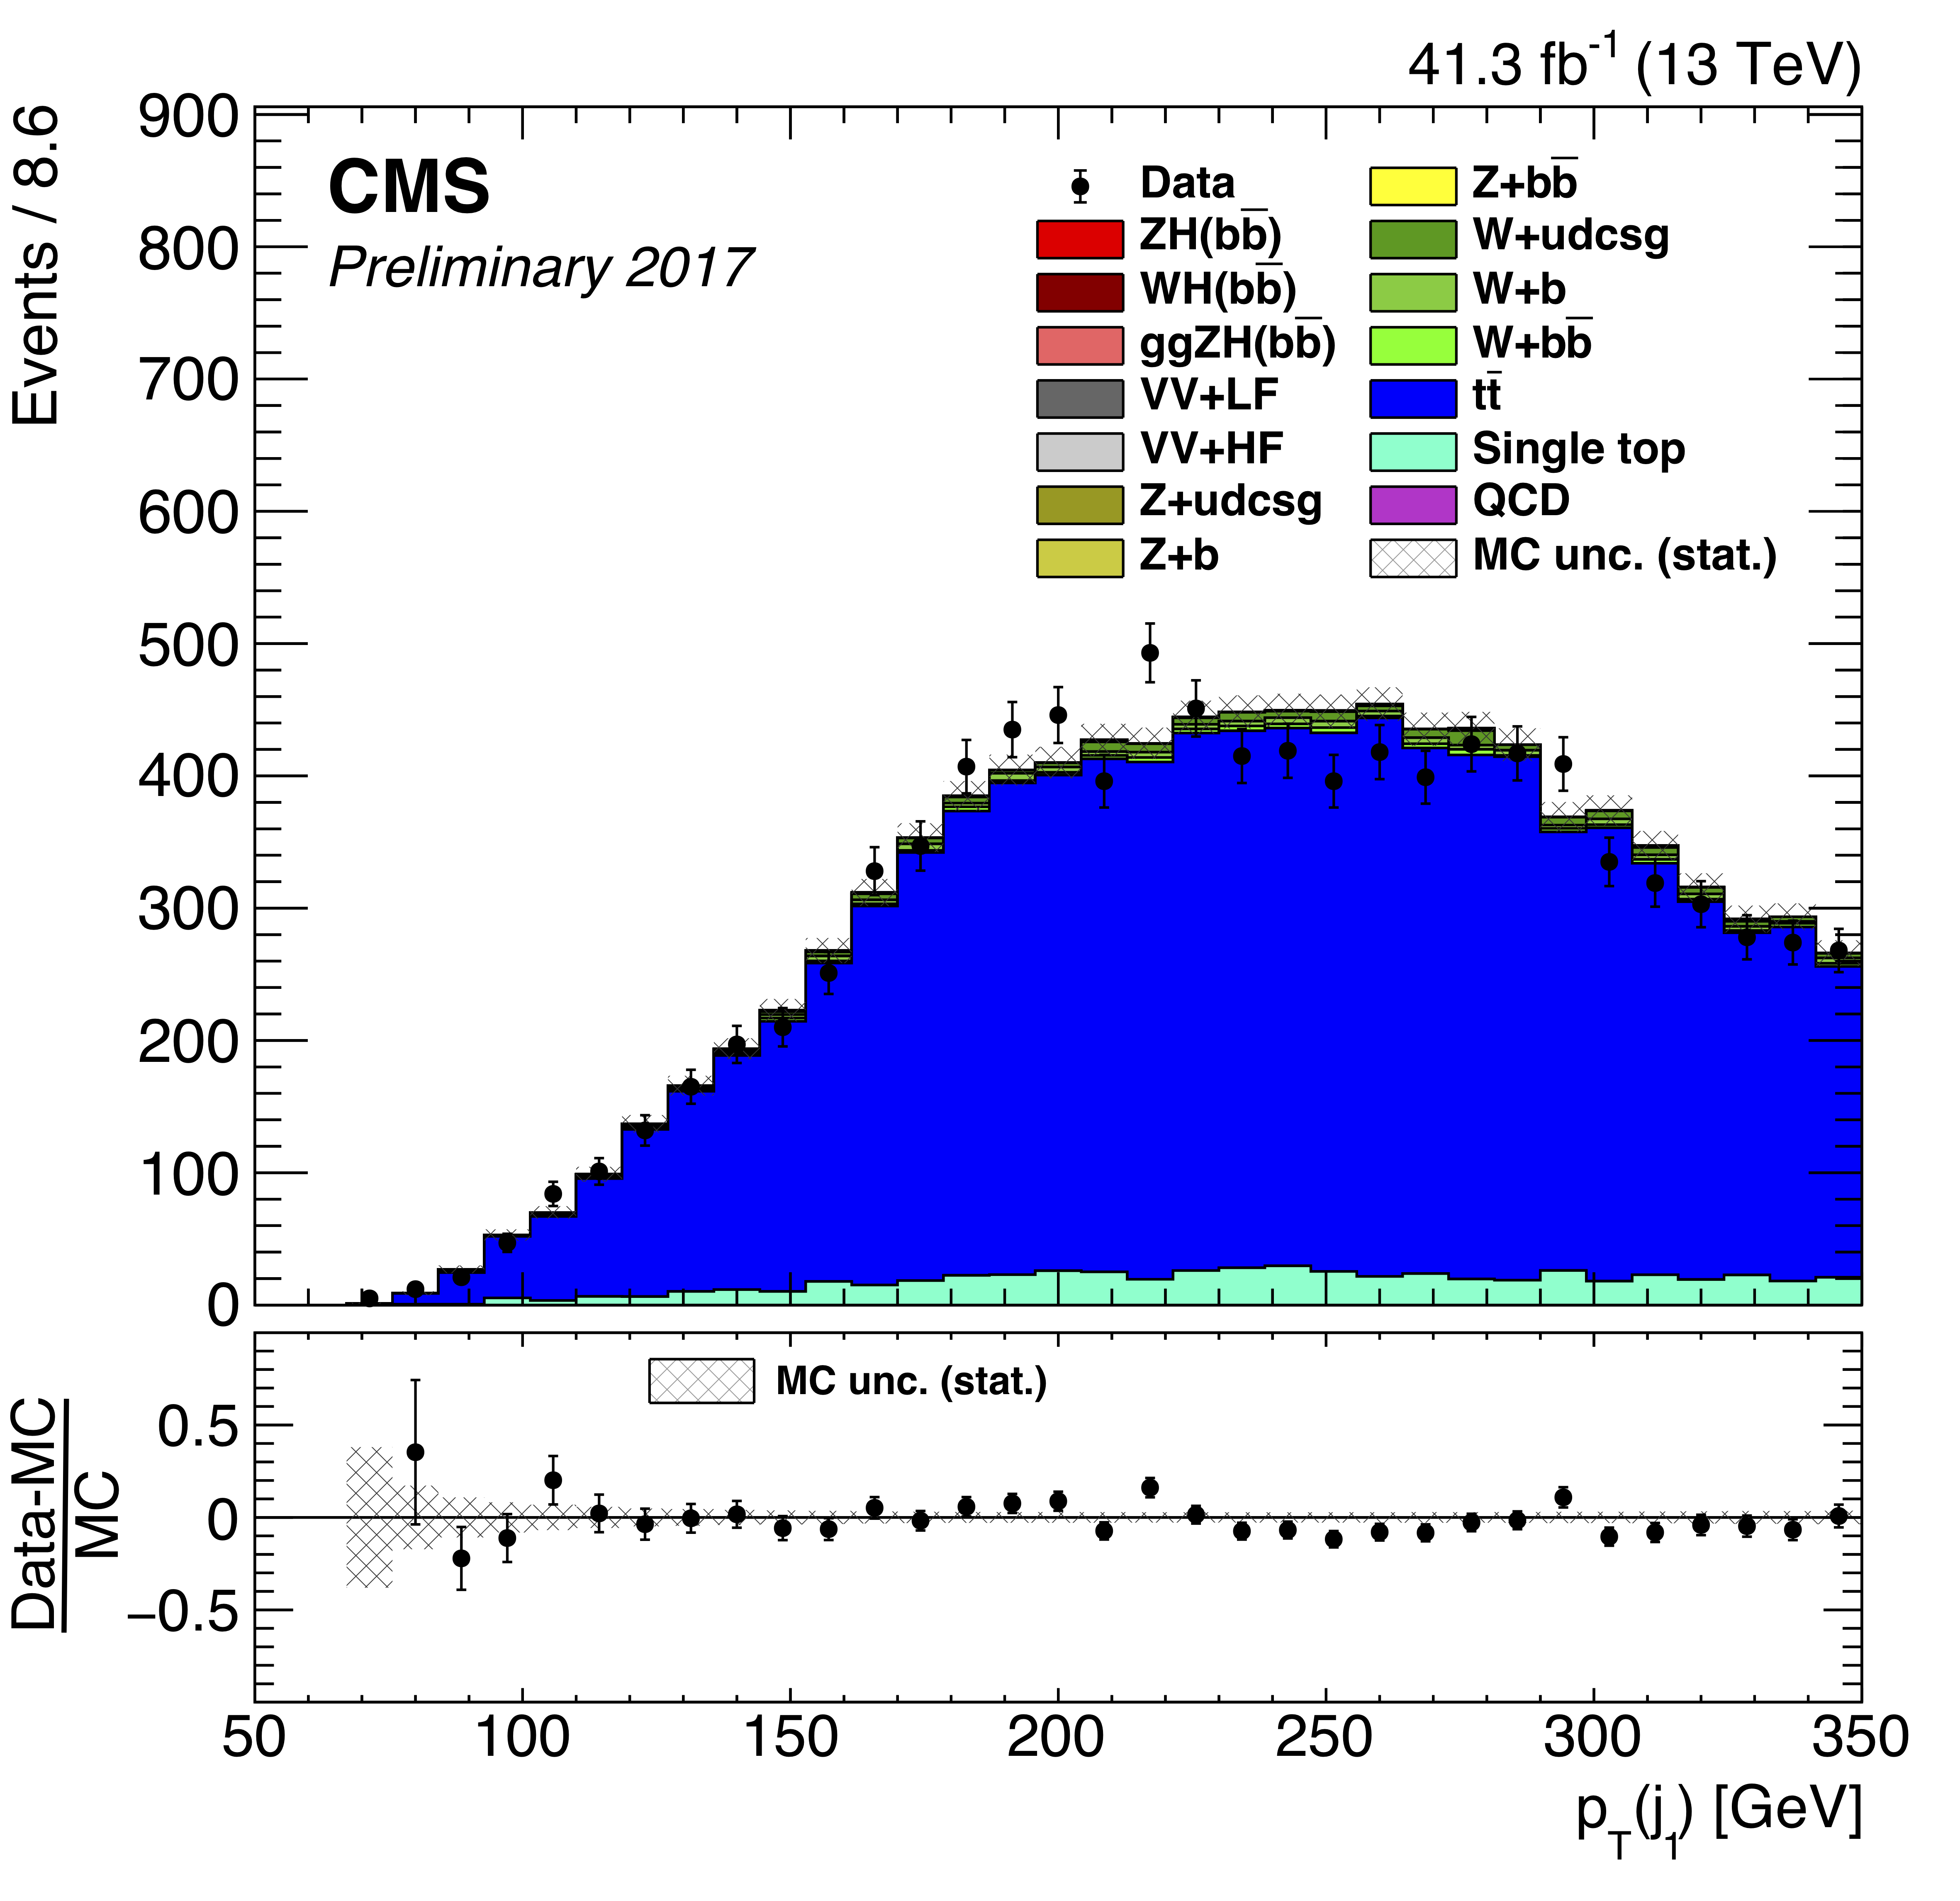
\includegraphics[width=0.4\linewidth]{images/CR_Znn_TT/hJets_leadingPt}}
    \subfigure [] {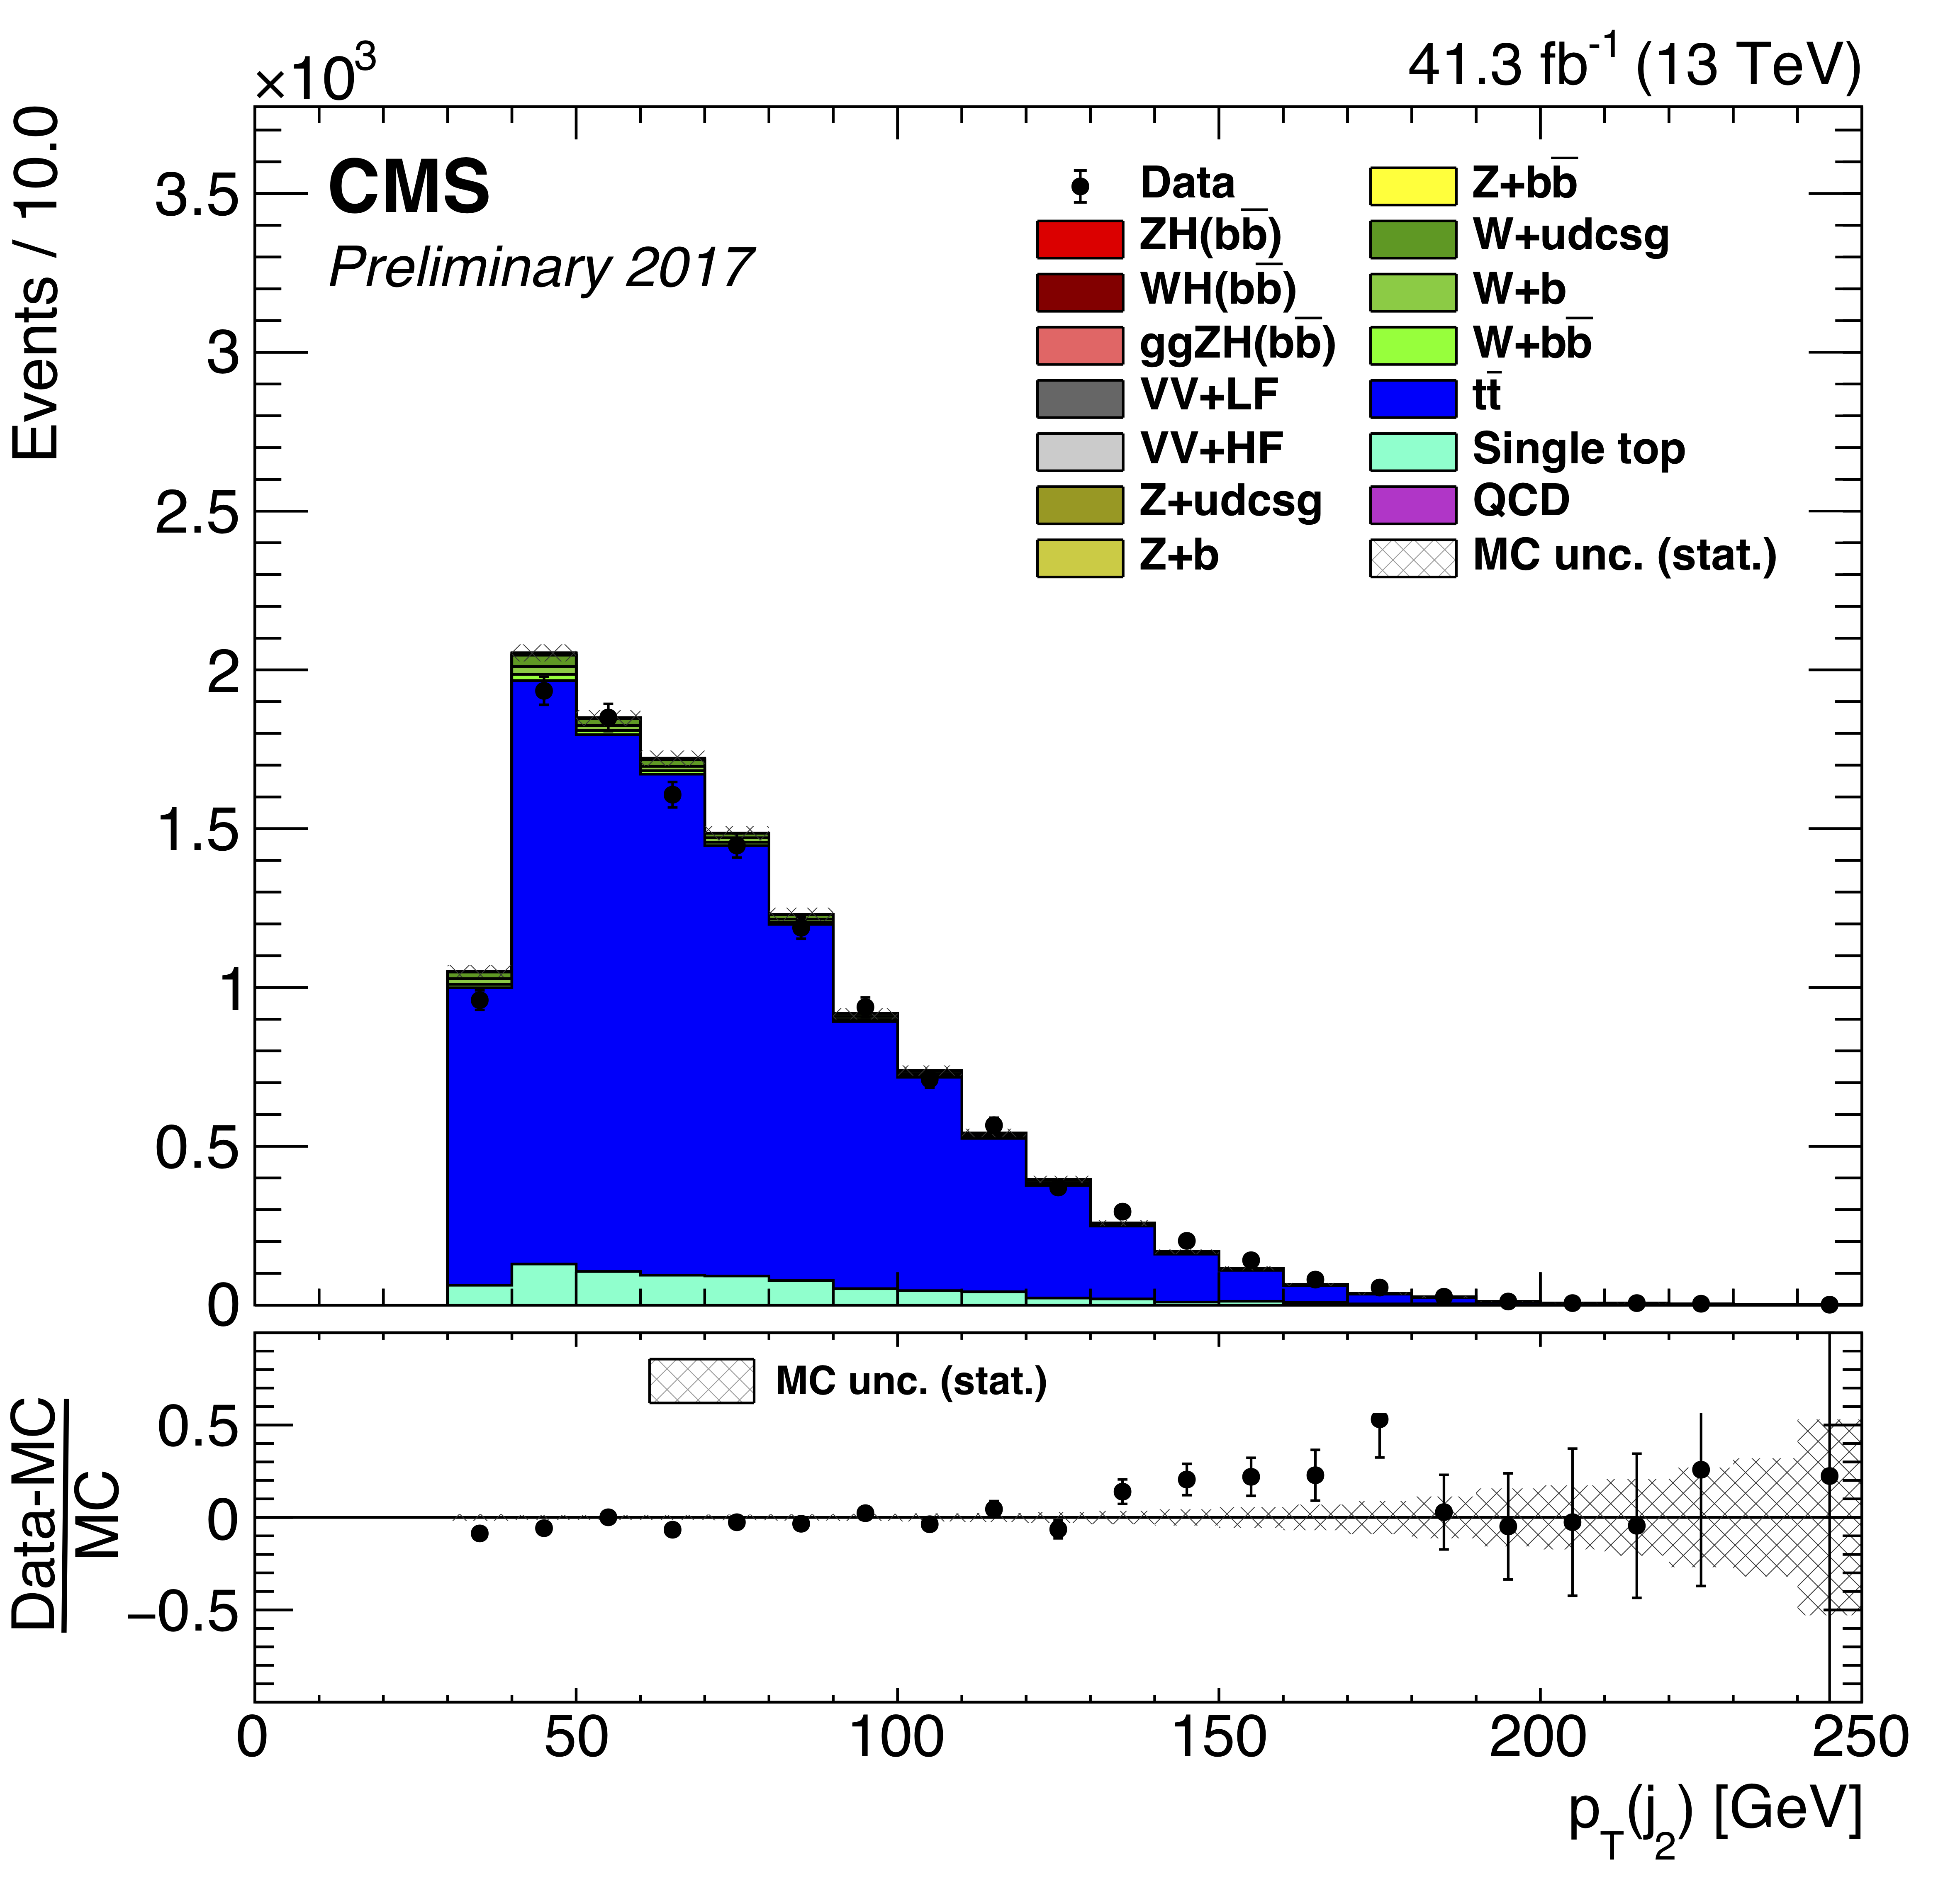
\includegraphics[width=0.4\linewidth]{images/CR_Znn_TT/hJets_subleadingPt}}
  }
  \caption[Higgs Candidate Distributions for the \ZnnH\ \qrkt\qrktbar\ Control Region]{The distributions of the Higgs boson candidate properties for the \qrkt\qrktbar\ control region of the \ZnnH\ channel: A) $m(jj)$, B) $\pT(jj)$, C) \btagmax, D) \btagmin, E) \pTjmax, F)  \pTjmin.}
  \label{fig:CR_Znn_TT_1}
\end{figure}


%\clearpage %remove this command if your appendix doesn't start with a landscaped page!!!!!
%\thispagestyle{plain}
%\begin{landscape}
%\begin{figure}
 
%  \begin{center}
%    
\includegraphics[width=6in]{images/LaTeX2e_logo.eps}
%    \caption{\LaTeX 2\ensuremath{\epsilon.} logo}\label{biglogo}
%  \end{center}
%\end{figure}
%\end{landscape}
 
 
%This is how a section should look if the first page is a landscape page.
%Lorem ipsum dolor sit amet, consectetuer adipiscing elit. Ut sit
%amet nulla. Integer mauris turpis, dapibus ac, auctor non, vehicula
%sit amet, magna. Suspendisse eu tellus. Etiam porta. Donec magna.
%Donec ut dui. In hac habitasse platea dictumst. Nullam suscipit, mi
%at adipiscing commodo, lorem erat scelerisque erat, non pulvinar leo
%mi eu metus. Phasellus id felis. Sed quam purus, molestie quis,
%ultrices nec, dictum at, magna. Proin viverra viverra ante.
